\section{Optymalizacja programu}
W celu określenia wydajności programu w kontekście wykorzystania dostępnych zasobów karty graficznej użyto narzędzia \textbf{NVIDIA Nsight Compute}. Pozwala ono na zbieranie wielu danych odnośnie wykonywanego programu i jego interakcji z kartą graficzną. Wiedza o tych interakcjach jest podstawą do prób optymalizacji programu. Wyniki przedstawiono poniżej.

\subsection{Wyniki programu profilującego}

Podstawowym badaniem przeprowadzanym przez narzędzie jest \textbf{GPU Speed Of Light}. To ogólne porównanie wykorzystanych zasobów obliczeniowych i pamięciowych do teoretycznego maximum parametru dla danej karty graficznej.\\
Na rysunku \ref{fig:speed_of_light} przedstawiono wyniki z działania tego narzędzia dla naszego programu.
\begin{figure}[H]
    \centering
    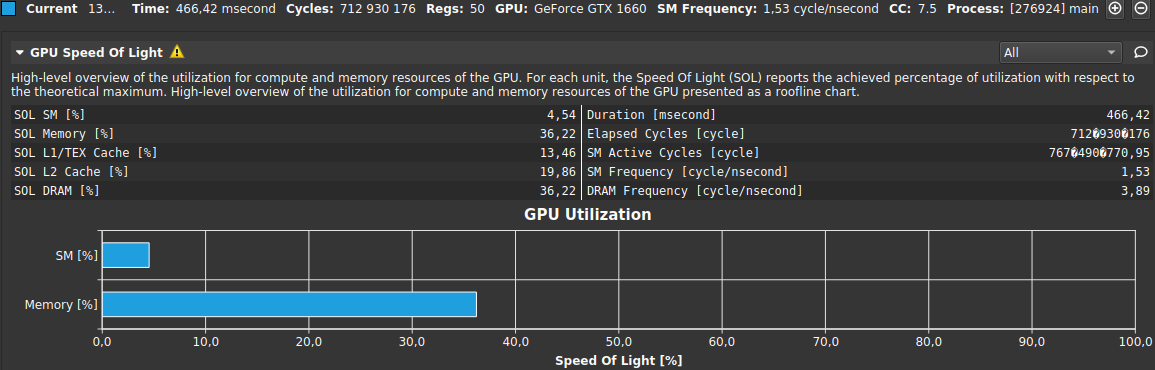
\includegraphics[width=\linewidth]{images/SpeedOfLight.png}
    \caption{Wyniki badania \textbf{GPU Speed Of Light}}
    \label{fig:speed_of_light}
\end{figure}
Widać, że wykorzystanie możliwości obliczeniowych karty graficznej to w tym przypadku ok. 4\%, a pamięci ok. 35\%.\\
Natomiast na rysunku \ref{fig:sm_analisys} przedstawiono treść ostrzeżenia znajdującego się w sekcji \textbf{Speed Of Light} oraz wyniki dokładniejszej analizy obciążenia procesorów strumieniowych.
\begin{figure}[H]
    \centering
    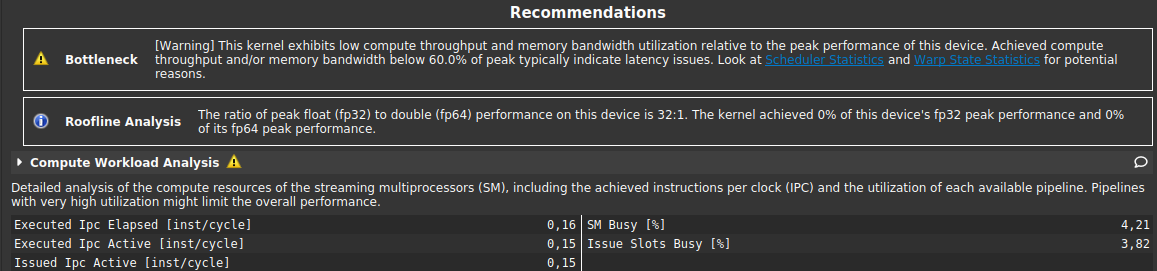
\includegraphics[width=\linewidth]{images/SMAnalysis.png}
    \caption{Wyniki badania \textbf{Compute Workload Analysis}}
    \label{fig:sm_analisys}
\end{figure}
Powyższe wyniki wskazują na to, że karta nie pracuje z pełną wydajnością. Wyniki tego badania jednak nie wskazują jasno, gdzie tracona jest skuteczność implementacji. Ostrzeżenie podpowiada, by sprawdzić wyniki badaniań \textbf{Scheduler Statistics} i \textbf{Warp State Statistics}. 

\begin{figure}[H]
    \centering
    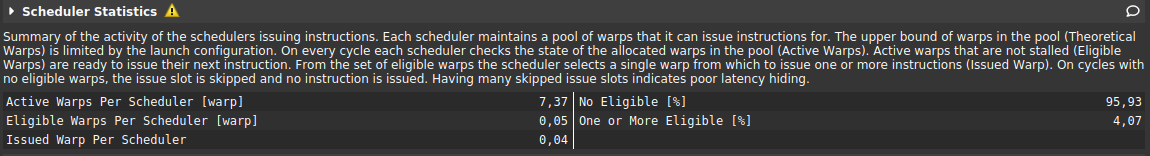
\includegraphics[width=\linewidth]{images/Scheduler.png}
    \caption{Wyniki badania \textbf{Scheduler Statistics}}
    \label{fig:scheduler}
\end{figure}

Na grafice \ref{fig:scheduler}. widać niskie wartości dwóch ostatnich pozycji w lewej kolumnie wyników, co wskazuje na małą średnią liczbę aktywowanych warp'ów na jeden cykl (\textit{Eligible Warps Per Scheduler}, \textit{Issued Warps Per Scheduler}). Liczba warp'ów znajdujących się w stanie aktywnym jest za to wysoka (dla tej architektury karty maksymalna ich liczba wynosi 8). Potwierdzają to także statystyki z prawych kolumn mówiące o wysokiej niedostępności warp'ów (\textit{No Egible} - 96\%). Takie wyniki mogą wskazywać na duże problemy związane z opóźnieniem dostępu do pamięci.

Wyniki badania \textbf{Warp State} pokazują także dość dużą średnią liczbę cykli na wykonaną jedną instrukcję programu.

\begin{figure}[H]
    \centering
    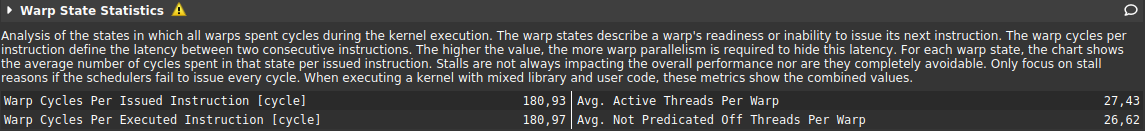
\includegraphics[width=\linewidth]{images/WarpState.png}
    \caption{Wyniki badania \textbf{Warp State Statistics}}
    \label{fig:warps}
\end{figure}

\subsection{Wnioski profilowania}

Powyższe wyniki wskazują jednoznacznie na słabe wykorzystanie przez program mocy \textbf{GPU}. Przyczyną tego jest potrzeba dostępu do różnych obszarów pamięci dla każdego wątku. Dostęp do pamięci globalnej (w niej przechowujemy przeszukiwany tekst) odbywa się dla każdego wątku pobierając zawsze 128-bitowy fragment pamięci. Jest on później zapisywany w pamięci współdzielonej, do której mają dostęp wątki z jednego warp'a. Jeśli kolejne wątki potrzebują danych ułożonych w pamięci sekwencyjne, to liczba dostępów do pamięci globalnej jest drastycznie mniejsza. Zastępowana jest dużo szybszym dostępem do pamięci współdcielonej, która ma czas dostępu porównywalny z czasem dostępu do rejestrów. Dużą liczbę odwołań do pamięci globalnej potwierdzają także dodaktowe komunikaty profilera, po wykonywaniu analizy wywołań poszczególnych instrukcji kodu. 

\begin{figure}[H]
    \centering
    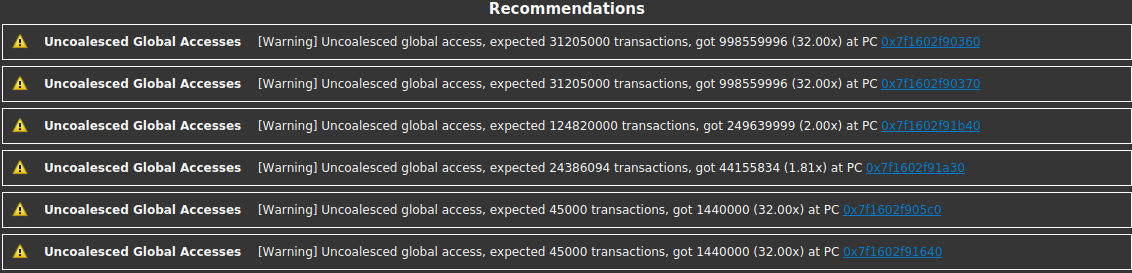
\includegraphics[width=\linewidth]{images/Warnings.png}
    \caption{Rekomendacje programu profilującego w sekcji \textbf{Source Counters}}
    \label{fig:warnings}
\end{figure}

Ostrzeżenia te mówią, o spodziewanej, optymistycznej liczbie dostępów do pamięci globalnej dla zadanej linii kodu, a rzeczywistym stanem. Różnice często są, w naszym przypadku, 32 krotne. Bezpośrednim powodem tego problemu jest struktura naszego programu. Kolejne wątki muszą mieć dostęp do stosunkowo odległych fragmentów przeszukiwanego tekstu. Aby zachować jednak charakter algorytmu Rabina-Karpa, tj.: obliczanie funkcji haszującej z wykorzystaniem wartości tejże funkcji dla poprzedniego okna tekstu, trzeba zachować przynajmniej lokalną sekwencyjność wykonywanego algorytmu. Najlepiej działa on, gdy sekwencje wyszukiwanych  Można się zastanowić, czy utrata wydajności spowodowana takim podejściem do problemu jest większa niż zyski spowodowane szybkim obliczaniem funkcji haszującej. Odpowiedzią na to pytanie byłoby porównanie naszej wersji algorytmu do równoległego, \say{naiwnego} przeszukiwania tekstu. W przypadku badania wykonanego dla optymistycznych przypadków, algorytm wykazał nawet 9-krotne przyspieszenie (rys. \ref{fig:chart_3}) w stosunku do przypadków pesymistycznych, dla których rozwiązanie degeneruje się do przeszukiwania \say{naiwnego}. Jeżeli implementacja \say{naiwna} miałaby być szybsza, musiałaby wykorzystywać zasoby karty graficznej przynajmniej kilkukrotnie lepiej niż obecny program.

%DAAAAAAMN!%